% siminos/gudorf/thesisProposal/done.tex
% $Author: mgudorf3 $ $Date: 2019-01-18 03:59:36 -0500 (Fri, 18 Jan 2019) $
\newpage
\section{Spatiotemporal \KSe}
\label{section:done}
The use of doubly periodic boundary conditions, $u(x,t) = u(x+L,t) = u(x,t+T) = u(x+L,t+T)$ for $x \in [0,L]$ and $t \in [0,T]$,
is constant through this work. These boundary conditions motivate
the use of a Fourier-Fourier basis (hereafter referred to as the \sFb\ ).
The most common and important term used in the following discussion is ``\spt\ \twot{}''.
This term will refer to a solution to the \KSe\ that is a 2-torus in configuration space due to the doubly-periodic boundary conditions.
A \rv\ \sFb\ will be used such that the scalar velocity field $u(x,t)$ has the following expansion,

\beq
\begin{aligned}
u(x,t) = \frac{1}{\sqrt{NM}}\sum_{n,m=0}^{N/2,M/2} \Big( & \nm{a}(\cos(\qm \conf)\cos(\wn \zeit)) + \nm{b}(\sin(\qm \conf)\cos(\wn \zeit))\\
                                    &+ \nm{c}(\cos(\qm \conf)\sin(\wn \zeit)) + \nm{d}(\sin(\qm \conf)\sin(\wn \zeit)) \Big)
\,.
\end{aligned}
\ee{sFb}

Let \Fuvec\ be defined as the vector composed of all \rv\ \spt\ Fourier coefficients, which is
assumed to be ordered in such a manner that the subseqeunt equations and definitions are logically consistent.
Substituting the Fourier expansion into \refeq{KS} yields a system of nonlinear algebraic equations,

\beq
(\Dt -\Dxx + \Dfourx) \Fuvec + \sum_{n',m'} \tilde{u}_{n-n',m-m'} \tilde{u}_{n,m} =0
\,,
\ee{KS_sFb_sum}

which depend explicitly on the \spt\ Fourier coefficients and implicitly on the scalar parameters $(T,L)$ through
the spectral differentiation operators $D_i$. For numerical accuracy and simplicity, a
\emph{pseudospectral} formulation of \refeq{KS_sFb_sum} is used,

\beq
(\Dt -\Dxx + \Dfourx) \Fuvec + \frac{1}{2} \Dx \F (\Fi(\Fuvec)^2)=0
\,.
\ee{KS_sFb}

The term ``pseudospectral'' refers to the specific manner in which the nonlinear term is calculated.
The operators in \refeq{KS_sFb}, \F\ and \Fi\ , represent the forward and backwards Fourier transforms, respectively.

\subsection{Spatiotemporal symmetries}
\label{subsubsection:symmetries}
The \KSe\ is equivariant under Galilean symmetry transformations,
\On{2} symmetry transformations in space, and \SOn{2} symmetry transformations in time.

Galilean transformations are defined by $u(x,t) \rightarrow u(x-vt,t)-v$,
where $v$ is an independent variable. This is the easiest symmetry to account for,
which is done by enforcing the following constraint for all solutions,
\[
\int u(t) \, \text{d}x = 0 \quad \forall t \in [0,T]
\,,
\]

which equates to constraining all spatiotemporal Fourier modes with spatial index $m=0$ to zero.
This constraint removes Galilean invariance from all further discussion; therefore, the focus shifts
to symmetries that can be represented by subgroups of the \spt\ symmetry group, $\On{2} \rtimes \SOn{2}$.

\subsubsection{Discrete symmetries}
Borrowing intuition from previous analysis of the \KSe{}, this formulation
will consider only two discrete symmetries,
spatial reflection symmetry and shift-reflection
(spatial reflection and half-cell time translation) symmetry\rf{BudCvi14,lanCvit07}.
For mathematical brevity, let $R_{\conf}$ and $R_{\conf} \tau_{1/2}$
denote spatial reflection and shift-reflection operations, respectively.
The action of spatial reflection is written,

\beq
R_{\conf}u(x,t) = -u(-x,t)
\eeq

and shift-reflection operation is written,

\beq
R_{\conf} \tau_{1/2} u(x,t) = -u(-x,t+\frac{T}{2})
\eeq

Solutions that display these symmetries satisfy the corresponding invariance conditions,

\beq
R_{\conf} \ufield - \ufield = 0 \,,
\ee{KSrefl}

\beq
R_{\conf} \tau_{\zeit} \ufield - \ufield = 0
\,.
\ee{KSsr}

When the \rv\ \sFb\ expansion \refeq{sFb} is substituted into \refeq{KSrefl} and \refeq{KSsr},
a set of conditions or ``selection rules'' that constrain
the \spt\ Fourier coefficients is produced. These selection rules can also be interpreted as definitions
for \emph{symmetry invariant subspaces}. Reflection invariance implies antisymmetric parity in space; therefore all spatially
symmetric modes are forced to be zero. Stated explicitly, reflection invariance implies,

\beq
\nm{a},\nm{b}= 0 \,,
\ee{reflectionrules}

Similarly, for shift-reflection symmetry,
the spatially symmetric modes must be antisymmetric in time, while spatially antisymmetric
modes must be symmetric in time (the time parity is with respect to $t=T/2$). Therefore the selection rules are given by,

\bea \label{shiftreflectionrules}
\nm{a},\nm{b} &=& 0 \, \mbox{for}\, n \, \mbox{even and} \, m=0 \continue
\nm{c},\nm{d} &=& 0 \, \mbox{for}\, n \, \mbox{odd and} \, m=0
\eea

It should be noted that shift-reflection symmetry is
prevalent in fluid dynamics calculations\rf{GHCW07,HGC08,KawKida01,Visw07b}, it has not
been discussed for either the \spt\ \KSe\ nor other \spt\ problems. In fact, the term
``\spt\ symmetry'' has not personally been observed in the literature.

\subsubsection{Continuous spatial translation symmetry}
The last remaining symmetry to be considered in this formulation is continuous spatial translation symmetry.
This manifests in \spt\ \twot\ solutions as a periodicity condition which depends on
both the period of the solution $T$ and spatial shift idiosyncratic to the solution, denoted by $g(\sigma) \in$ \SOn{2},

\beq
u(x,t) = g \circ u(x,t+T_p) \,
\ee{ks_rpo}

$\sigma$ denotes the idiosyncratic spatial translation (``the shift'') of a solution.
Two possible methods to deal with this continuous symmetry are: quotienting the symmetry
via first Fourier mode slice\rf{BudCvi14,BudCvi15} or performing a coordinate transformation
that maps the \spt\ field into a reference frame in which it is periodic, called the
``mean-velocity frame''.
The difficulty of the \spt\ implementation of the slicing method is sufficient enough to
warrant use of the mean-velocity frame method.

The mean-velocity frame is mathematically equivalent to using the ansatz (written in complex representation for brevity),
\beq
a_m(t) =  e^{-\frac{2 \pi \ii m \sigma t}{LT}}\sum_{n,m} \umn e^{\ii (\qm \conf + \wn \zeit)}
\,.
\ee{ks_mvf_ansatz}

This ansatz results in a modified equation due to the time derivative of the exponential prefactor,

\beq
(\Dt -\Dxx + \Dfourx + \Sop) \Fuvec + \frac{1}{2} \Dx \F (\Fi(\Fuvec)^2)=0
\,.
\ee{KS_mvf}

This ansatz and subsequent equation modification are sufficient to find \twots\ with
spatial translation symmetry. In contrast to discrete symmetries, there are no selection rules
defined by this symmetry.
Now that all considered symmetries and their subsequent equations have been derived the next step
is to develop numerical methods to solve said equations.

\section{Numerical methods}
\label{section:methods}
This section derives and describes the various numerical methods and algorithms used
to find \twot\ solutions of the \KSe{}. While this is the lion's share of the work, specific details
will be avoided as much as possible.

The structure of this section is as follows: first, initial condition generation is described
in \refsect{subsection:init}. Second, a powerful yet sometimes prohibitively expensive
method called the ``damped Gauss-Newton'' method (dGN)
is described first in \refsect{subsection:newton}.
Finally, two faster but less powerful methods (in terms of rate of convergence) are derived.
These are the ``adjoint descent method''\rf{Faraz15} and GMRES or ``general minimized residual method''\rf{Saad1986},
which are described in \refsect{subsection:adjoint} and \refsect{subsection:GMRES}, respectively.


\subsection{Notation}
First, let us define some notation that will be convenient for the following discussion.
The \emph{state space vector} $\mathbf{u}$ denotes a vector that contains all computational variables:
the spatiotemporal Fourier modes, the period, spatial domain size,
and the \SOn{2} parameter $\sigma$.

\beq
\mathbf{u} = (\Fuvec,T,L,\sigma{}) \,
\eeq

The parameter $\sigma$ is only present when the \textit{a priori}
assumption of continuous symmetry is made.
Likewise, if we decide to keep either $L$ or $T$ fixed then the respective variable
would no longer be present in $\mathbf{u}$.

If the \KSe\ is represented as a vector function $\mathbf{F}$, then the
root-finding problem can be trivially rewritten as,

\beq
\mathbf{F}(\mathbf{u}) = \mathbf{0} \,,
\eeq

A useful mathematical construction is the so-called \emph{cost function}, written,

\beq
I(\mathbf{u}) = \frac{1}{2}||\mathbf{F}(\mathbf{u})||^2
\,,
\ee{cost_functional}

where the norm is the $L_2$ norm. The cost function is a non-negative scalar function
that only equals zero when $\mathbf{F}(\mathbf{u})=0$. Therefore, solving
$\mathbf{F}=\mathbf{0}$ is equivalent to solving for $I=0$.

Last is the derivation of the equations used in the damped Gauss-Newton method,
Let $\mathbf{u}* = \mathbf{u}+ \delta \mathbf{u}$
be a root of $\mathbf{F}(\mathbf{u})$ such that $\mathbf{F}(\mathbf{u}^*)=0$, then,

\bea \label{eqn:newton}
\mathbf{F}(\mathbf{u} + \delta \mathbf{u}) &\approx& \mathbf{F}(\mathbf{u}) + \frac{\partial \mathbf{F}}{\partial \mathbf{u}} (\delta \mathbf{u}) \continue
\mathbf{F}(\mathbf{u}^*) &\approx& \mathbf{F}(\mathbf{u}) + \frac{\partial \mathbf{F}}{\partial \mathbf{u}} (\delta \mathbf{u})\continue
0 &\approx& \mathbf{F}(\mathbf{u}) + \frac{\partial \mathbf{F}}{\partial \mathbf{u}} \delta \mathbf{u} \continue
-\mathbf{F}(\mathbf{u})  &\approx& \frac{\partial \mathbf{F}}{\partial \mathbf{u}} \delta \mathbf{u} \,.
\eea

The last equation in \refeq{eqn:newton} will be referred to as the ``Newton equation''.
The matrix $\frac{\partial \mathbf{F}}{\partial \mathbf{u}}$
will be called the ``Jacobian matrix'' and denoted by $J$.

\subsection{Initial condition generation}
\label{subsection:init}

Initial condition generation is often overlooked
as a place for improvement due to lack of possible methods.
The algorithm described in this section is only afforded to
a spatiotemporal formulation
and has many computational advantages over the conventional
``close recurrence'' procedure for producing initial conditions
used in \refrefs{ChaKer12,STGS18}.

Typically, the close recurrence method
is comprised of storing a time-integrated series of points. Once the time integration finishes,
the pointwise $L_2$ norm between different time series points are calculated. The
minima of this pointwise calculation are taken to indicate trajectory segments
that nearly close on themselves which approximate periodic orbits. The main disadvantage
is that the computational cost increases substantially in the limit of large spatial domains.

The spatiotemporal initial condition generation method initializes an entire
spatiotemporal domain at once by randomly assigning values to the \rv\ Fourier
mode coefficients. After the computational modes are initialized, spatial and temporal scales
are imposed via manipulation of the spectrum of Fourier modes. This procedure guarantees
that the initial condition not only has the desired scales but is
also doubly periodic and smooth. Some example initial conditions are displayed in \reffig{fig:MNGspacetimeinit}.

\begin{figure} %[ht]
\centering
\begin{minipage}[height=.25\textheight]{.25\textwidth}
\centering \small{\texttt{(a)}}
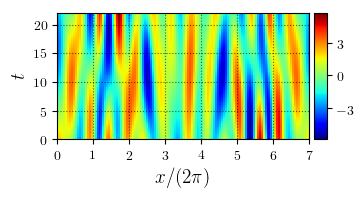
\includegraphics[width=\textwidth,height=.25\textheight]{MNG_ppo_init}
\end{minipage}
\begin{minipage}[height=.25\textheight]{.25\textwidth}
\centering \small{\texttt{(b)}}
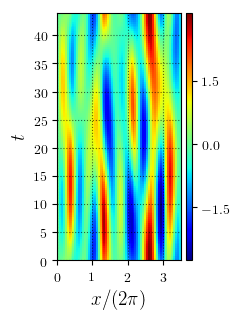
\includegraphics[width=\textwidth,height=.25\textheight]{MNG_anti_init}
\end{minipage}
\begin{minipage}[height=.25\textheight]{.25\textwidth}
\centering \small{\texttt{(c)}}
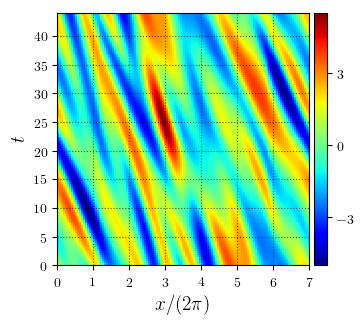
\includegraphics[width=\textwidth,height=.25\textheight]{MNG_rpo_init}
\end{minipage}
\caption{ \label{fig:MNGspacetimeinit}
Example spatiotemporal initial conditions for three symmetry types,
(a) shift-reflection,
(b) reflection,
(c) spatial translation.
}
\end{figure}


\subsection{Damped Gauss-Newton method}
\label{subsection:newton}

The first numerical method falls under the broad category of ``Newton methods''. This
method directly solves the nonlinear root finding problem $\mathbf{F}(\mathbf{u})=0$ associated with the Newton equation,

\beq
\begin{bmatrix}
\frac{\partial \mathbf{F}}{\partial \Fuvec\ } & \frac{\partial \mathbf{F}}{\partial T} & \frac{\partial \mathbf{F}}{\partial L} & \frac{\partial \mathbf{F}}{\partial \sigma}
\end{bmatrix}
\delta \mathbf{u}
=
- \mathbf{F}(\mathbf{u})\,.
\ee{leastsquaresNewton}

The Newton equation \refeq{leastsquaresNewton} is an over-determined (rectangular) system of equations.
This requires us to either provide constraints to make the system square, or solve the system in a least squares manner.
We elect to solve the least-squares problem, using what we call the ``damped Gauss-Newton'' method (dGN).
``Gauss-Newton'' implies that \refeq{leastsquaresNewton} is solved directly by calculating the Moore-Penrose pseudoinverse of the
linear system, $A^{+} \equiv (A^{\top}A)^{-1}A^{\top}$, such that the solution is given by $\delta x = A^{+}(-\mathbf{F}(\mathbf{u}))$.

The qualifier ``damping'' denotes the introduction of a scalar parameter $d$ that is
decreased until $I(\mathbf{u} + d(\delta \mathbf{u})) < I(\mathbf{u})$, is satisfied. A minimum bound $\epsilon$
is introduced such that  $\epsilon < d < 1$. This ensures the norm of the solution does not become too small.
In practice, for each solve of the Newton equation,
$d_0 = 1$ and is divided by $2$ until  $I(\mathbf{u} + \frac{1}{2^k}(\delta \mathbf{u})) < I(\mathbf{u})$ or until
$k=10$.

\subsection{Adjoint descent method}
\label{subsection:adjoint}
The previous section discussed a direct method for solving the Newton equation. While powerful,
the matrix $J$ must be explicitly formed so that the pseudoinverse can be calculated. This becomes expensive, sometimes prohibitively so,
as the dimension of the state vector approaches $\text{dim}[\mathbf{{u}}] \approx \mathcal{O}(10^4)$.
Therefore, numerical methods that do not rely on explicit matrix construction are required.
The first such method to be discussed is called the ``adjoint descent method''\rf{Faraz15}.

The derivation of the adjoint descent method begins by taking a
derivative of the cost function \refeq{cost_functional} with respect to
a continuous fictitious time, denoted by $\tau$. $\tau$ is a continuous variable which
parameterizes the numerical method such that
as $\tau \rightarrow \infty$, the cost function converges to zero $I(\tau) \rightarrow 0$.

\beq
\partial_{\tau} I(\mathbf{u}) = J^{\top}F \,\partial_{\tau}\mathbf{u}
\,,
\ee{general_descent}

Eq.~\refeq{general_descent} includes an implicit choice for $\partial_{\tau}\mathbf{u}$.
A useful choice is one that guarantees a monotonically decrease of the cost
function. One specific choice,

\beq
\partial_{\tau}\mathbf{u} = - J^{\top}F
\,,
\ee{adjoint_descent_direction}

will be referred to as the ``adjoint direction''. This choice ensures that the cost function
is monotonically decreasing, as can be seen by,

\beq
\partial_{\tau} I(\mathbf{u}) = -||J^{\top}F||^2
\,,
\ee{adjoint_descent}

where the right hand side is a strictly non-negative function.
The adjoint descent method can be summarized
simply as numerical integration in the adjoint descent direction.

\subsection{GMRES}
\label{subsection:GMRES}
Yet another class of numerical methods implemented and utilized in this work are \textit{iterative methods}.
A very coarse description of iterative methods is that they are numerical methods that produce a sequence
of approximate solutions $x_k$ to linear system $Ax=b$ until some required tolerance or accuracy is achieved.

A common iterative method that is used for nonsymmetric matrices is known as GMRES\rf{Saad1986}.
GMRES falls under the broad category of Krylov subspace methods and has previously
been used to find time invariant solutions in fluid dynamics\rf{Visw08,ChanKers13}.
GMRES is comprised of two primary subroutines: Arnoldi iteration and a least-squares problem
constrained to a Krylov subspace.
Arnoldi iteration produces a Krylov subspace by successive matrix multiplication
and orthonormalization via modified Graham-Schmidt method. The original
optimization problem $||Ax-b||=0$ combined with the Arnoldi iteration recurrence relation,

\beq
A Q_k = Q_{k+1} H_k \,.
\ee{arnoldirecur}

leads to the GMRES equation,

\bea
\label{eqn:GMRES}
||Ax-b|| &=& ||A Q_k y-b|| \continue
    &=& ||Q_{k+1} H_k y-b|| \continue
    &=& ||H_k y-Q_{k+1}^{T}b|| \continue
    &=& ||H_k y-\beta e_1|| \quad \mbox{where,} \continue
\beta &=& ||b|| \,,
\eea

where $e_1$ is the unit vector whose first element is $1$, and is of dimension $k+1$.
The ``GMRES solution'' $y$, is a vector that minimizes the norm of $||H_k y - \beta e_1||$.

\section{Current results}
\label{section:results}
The numerical methods previously described are combined to create hybrid methods to find new
\spt\ \twot\ solutions to the \KSe{}. The most common and effective combination for finding solutions from experience is the combination of adjoint descent
from \refsect{subsection:adjoint} with the damped Gauss-Newton method of \refsect{subsection:newton}.

\subsection{Collection of new solutions}
\label{subsection:solutions}
A relatively large ($\mathcal{O}(10^3)$) number of new
\twot\ solutions have been found. \refFig{fig:MNGspacetimefinal} displays the solutions that
the example initial conditions, displayed in \reffig{fig:MNGspacetimeinit}, converge to. This convergence
proves that the \spt\ initial condition generation method from \refsect{subsection:init} is indeed viable.

\begin{figure} %[ht]
\centering
\begin{minipage}[height=.25\textheight]{.25\textwidth}
\centering \small{\texttt{(a)}}
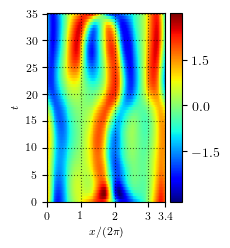
\includegraphics[width=\textwidth,height=.25\textheight]{MNG_ppo_fin}
\end{minipage}
\begin{minipage}[height=.25\textheight]{.25\textwidth}
\centering \small{\texttt{(b)}}
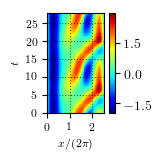
\includegraphics[width=\textwidth,height=.25\textheight]{MNG_anti_fin}
\end{minipage}
\begin{minipage}[height=.25\textheight]{.25\textwidth}
\centering \small{\texttt{(c)}}
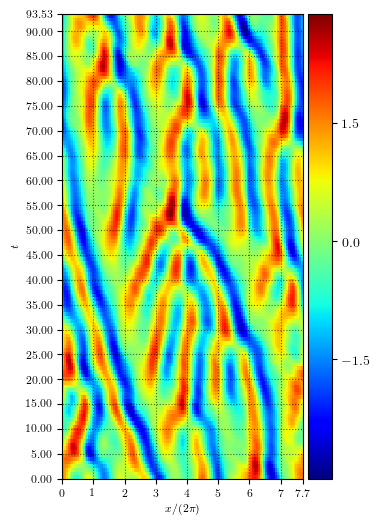
\includegraphics[width=\textwidth,height=.25\textheight]{MNG_rpo_fin}
\end{minipage}
\caption{ \label{fig:MNGspacetimefinal}
Examples of converged spatiotemporal solutions, the initial
conditions used are the \spt\ scalar fields from \reffig{fig:MNGspacetimeinit}. They have
symmetries,
(a) shift-reflection,
(b) reflection,
(c) spatial translation.
}
\end{figure}


\subsection{Spatiotemporal symbolic dynamics and tiling}
\label{subsection:tiles}
One goal of this work is to develop a \spt\ symbolic dynamics but this is only worthwhile if
the symbolic dynamics is simple enough to be useful.
The term `` \spt\ tile'', or just ``tile'' is used to describe \spt\ solutions that are
believed to be members of the \spt\ symbolic dynamic alphabet. The name ``tile'' was chosen to appeal
to the intuition on how tiles are combined. The simplicity of the symbolic
dynamics would be determined by the number of unique tile solutions as well as the
set of rules that determine admissible symbolic combinations.

The new collection of converged solutions described in \refsect{subsection:solutions}
is assumed to adequately sample the overall space of solutions such that all
\spt\ tiles can be found within. Patterns
that appear frequently within the collection of solutions are likely candidates for \spt\ tiles.
With this in mind, a collection of guess tiles was produced by manually scanning the database of new
solutions by eye and picking out the most common patterns.
These guesses are displayed in \reffig{fig:MNGtilescrude}.

\begin{figure} %[ht]
\centering
\begin{minipage}[height=.15\textheight]{.15\textwidth}
\centering \small{\texttt{(a)}}
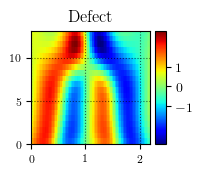
\includegraphics[width=\textwidth,height=.15\textheight]{MNG_defect}
\end{minipage}
\begin{minipage}[height=.15\textheight]{.15\textwidth}
\centering \small{\texttt{(b)}}
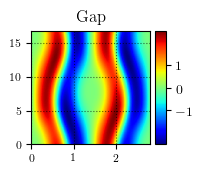
\includegraphics[width=\textwidth,height=.15\textheight]{MNG_gap}
\end{minipage}
\begin{minipage}[height=.15\textheight]{.15\textwidth}
\centering \small{\texttt{(c)}}
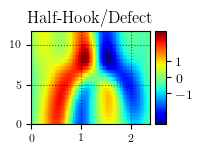
\includegraphics[width=\textwidth,height=.15\textheight]{MNG_half}
\end{minipage}
\begin{minipage}[height=.15\textheight]{.15\textwidth}
\centering \small{\texttt{(d)}}
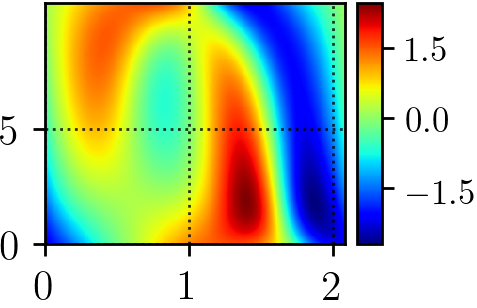
\includegraphics[width=\textwidth,height=.15\textheight]{MNG_hook}
\end{minipage}
\begin{minipage}[height=.15\textheight]{.15\textwidth}
\centering \small{\texttt{(e)}}
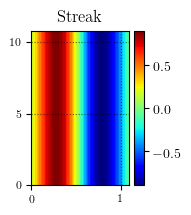
\includegraphics[width=\textwidth,height=.15\textheight]{MNG_streak}
\end{minipage}
\caption{ \label{fig:MNGtilescrude}
Guess ``tiles'' which were named:
(a) defect,(b) gap,(c) half-defect,(d) hook,(e) streak.
}
\end{figure}

To qualitatively demonstrate the purpose of the \spt\ tiles, the set of images from \reffig{fig:MNGtilescrude}
was used to very crudely approximate a known \spt\ solution. This was mainly a test to see if
the set of tiles in \reffig{fig:MNGtilescrude} was sufficiently large enough; if a pattern was
missing from our collection it would imply we need to search more thoroughly.
The approximation produced by cutting and pasting the images of guess tiles from \reffig{fig:MNGtilescrude}
and the ``target solution'' are compared in \reffig{fig:MNGfrankensteinconcept}. The approximation was constructed
using only three images.

\begin{figure} %[ht]
\centering
\begin{minipage}[height=.3\textheight]{.3\textwidth}
\centering \small{\texttt{(a)}}
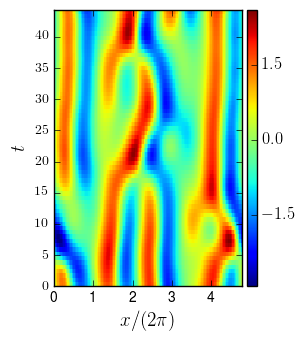
\includegraphics[width=\textwidth,height=.25\textheight]{MNG_ppo_L30_T44}
\end{minipage}
\begin{minipage}[height=.2\textheight]{.2\textwidth}
\centering \small{\texttt{(b)}}
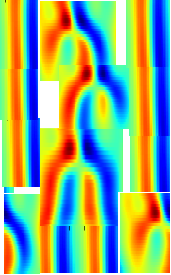
\includegraphics[width=\textwidth,height=.2\textheight]{MNG_ppo_frankenstein}
\end{minipage}
\caption{ \label{fig:MNGfrankensteinconcept}
Qualitative example of how one might build larger \spt\ solutions from a
library of small solutions. (a) A converged \twot\ solution with
shift-reflect symmetry; (b) An image thrown together using only a few
subdomains that attempts to capture the behavior of (a).
}
\end{figure}

\begin{figure} %[ht]
\centering
\begin{minipage}[height=.15\textheight]{.15\textwidth}
\centering \small{\texttt{(a)}}
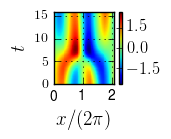
\includegraphics[width=\textwidth,height=.15\textheight]{MNG_defect_final}
\end{minipage}
\begin{minipage}[height=.15\textheight]{.15\textwidth}
\centering \small{\texttt{(b)}}
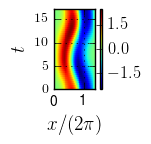
\includegraphics[width=\textwidth,height=.15\textheight]{MNG_gap_final}
\end{minipage}
\begin{minipage}[height=.15\textheight]{.15\textwidth}
\centering \small{\texttt{(c)}}
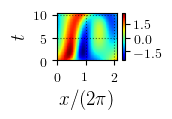
\includegraphics[width=\textwidth,height=.15\textheight]{MNG_hook_final}
\end{minipage}
\begin{minipage}[height=.15\textheight]{.15\textwidth}
\centering \small{\texttt{(d)}}
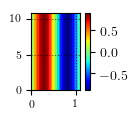
\includegraphics[width=\textwidth,height=.15\textheight]{MNG_streak_final}
\end{minipage}
\caption{ \label{fig:MNGsubdomainfinal}
Numerically converged \spt\ tiles:
(a)defect, (b)gap, (c)hook, (d)streak.
}
\end{figure}

The four tile guesses that converged numerically
are displayed in \reffig{fig:MNGsubdomainfinal}.
Of these four \spt\ tiles, three were determined to be unique.
The reduction from four to three tiles was the result of a
comparison of the ``defect'' and ``hook'' tiles. Numerical continuation was used to match the
domain sizes of the two tiles, after which the translational symmetries were
quotiented to ensure that they were indeed the same solution.
Visual comparison of the solutions displayed in \reffig{fig:MNGhookdefectcomparison}
seems sufficient enough to claim that the two tiles are indeed identical.

\begin{figure} %[ht]
\centering
\begin{minipage}[height=.45\textheight]{.45\textwidth}
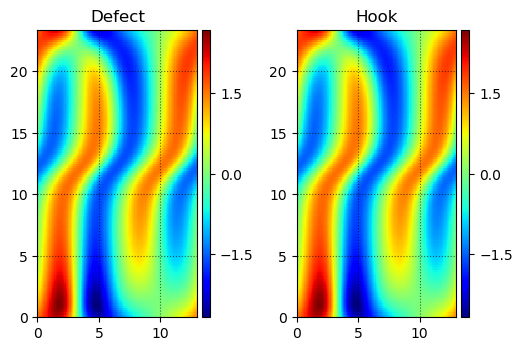
\includegraphics[width=\textwidth,height=.25\textheight]{MNG_hookdefect_comparison}
\end{minipage}
\caption{ \label{fig:MNGhookdefectcomparison}
Spatiotemporal tiles: (left) ``defect'' tile, (right) ``hook'' tile. The tiles have been
 numerically continued to the same domain size $\tilde{L} \approx
2.06 $. Spatial and temporal translational symmetries have been
quotiented via first Fourier mode slice\rf{BudCvi14} for spatial
translations
and phase fixing for time translations.
}
\end{figure}

The ability to numerically continue \spt\ tiles indicates
that the tiles exist in continuous families. Alternatively, tiles exist on deformable \spt\ domains, determined by the parameters, $T,L$ as opposed to static, rigid domains.
These families actually offer a useful explanation for the overlooked fact that continuous families of \spt\ \twots\ exist.
The proposed reconciliation between symbolic dynamics and continuous families of solutions is that solutions each have a unique and constant symbolic representation but the deformability
of the tiles allows solutions to exist as continuous families.
One foreseeable problem;however, is that if the admissibility of tile combinations
depends on the tiles' parameter values, the grammar might be hopelessly complex.

Acquiring a set of tiles is in and of itself not very useful, their utility is dependent on their ability to construct larger \spt\ solutions.
As a proof of concept, the qualitative tiling displayed in \reffig{fig:MNGfrankensteinconcept} is
now quantitatively constructed and converged numerically.
Visual inspection was used to determine the specific tiles and subdomains used to construct the initial conditions.
The symbolic representation and \spt\ scalar fields
of the two initial conditions are displayed in \reffig{fig:MNGsymbolsfail} and \reffig{fig:MNGsymbolsconverge}
Both of these initial conditions converged numerically to different \spt\ \twots{}.
The second attempt is believed to be identical to the targeted solution (up to small
time translation). All three numerically
converged solutions are displayed in \reffig{fig:MNGsymbolsconverged}.

\begin{figure} %[ht]
\centering
\begin{minipage}[height=.3\textheight]{.3\textwidth}
\centering \small{\texttt{(a)}}
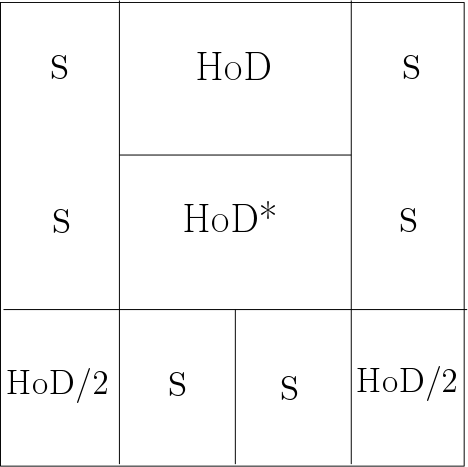
\includegraphics[width=\textwidth,height=.3\textheight]{MNG_incorrect_symbdyn}
\end{minipage}
\begin{minipage}[height=.35\textheight]{.35\textwidth}
\centering \small{\texttt{(b)}}
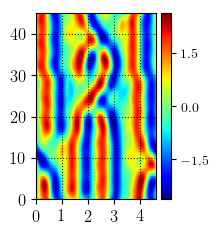
\includegraphics[width=\textwidth,height=.35\textheight]{MNG_ppo_tiling_init_0}
\end{minipage}
\caption{ \label{fig:MNGsymbolsfail}
Initial condition attempting to reconstruct a known solution.
The initial condition is displayed in both (a) \spt\ symbolic dynamical representation
and (b)\spt\ scalar field representation. This initial condition converged but not
to the desired solution
}
\end{figure}

\begin{figure} %[ht]
\centering
\begin{minipage}[height=.3\textheight]{.3\textwidth}
\centering \small{\texttt{(a)}}
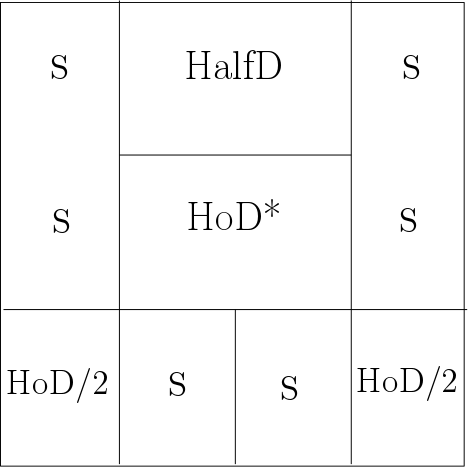
\includegraphics[width=\textwidth,height=.3\textheight]{MNG_correct_symbdyn}
\end{minipage}
\begin{minipage}[height=.35\textheight]{.35\textwidth}
\centering \small{\texttt{(b)}}
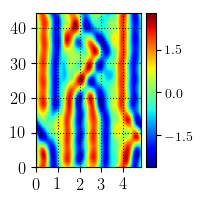
\includegraphics[width=\textwidth,height=.35\textheight]{MNG_ppo_tiling_init_1}
\end{minipage}
\caption{ \label{fig:MNGsymbolsconverge}
Initial condition attempting to reconstruct a known solution.
The initial condition is displayed in both (a) \spt\ symbolic dynamical representation
and (b)\spt\ scalar field representation. This initial condition converged
to the desired solution
}
\end{figure}


\begin{figure} %[ht]
\centering
\begin{minipage}[height=.25\textheight]{.25\textwidth}
\centering \small{\texttt{(a)}}
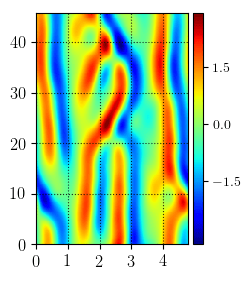
\includegraphics[width=\textwidth,height=.25\textheight]{MNG_ppo_tiling_final_0}
\end{minipage}
\begin{minipage}[height=.25\textheight]{.25\textwidth}
\centering \small{\texttt{(b)}}
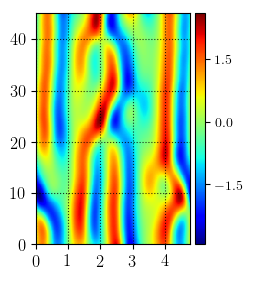
\includegraphics[width=\textwidth,height=.25\textheight]{MNG_ppo_tiling_final_1}
\end{minipage}
\begin{minipage}[height=.25\textheight]{.25\textwidth}
\centering \small{\texttt{(c)}}
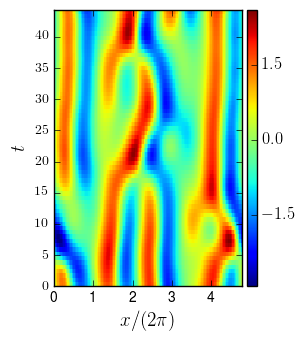
\includegraphics[width=\textwidth,height=.25\textheight]{MNG_ppo_L30_T44}
\end{minipage}
\caption{\label{fig:MNGsymbolsconverged}
(a)Numerically converged \spt\ \twot\ attained by numerically converging the initial condition (a) from \reffig{fig:MNGsymbolsfail}.
(b)Numerically converged \spt\ \twot\ attained by numerically converging the initial condition (c) from \reffig{fig:MNGsymbolsconverge}.
(c)Targeted solution. By visual inspection the converged solution (b) is equivalent to (c).
}
\end{figure}


\subsection{Spatiotemporal gluing}
It was shown in \reffig{fig:MNGsymbolsconverged} that an approximate \spt\ symbolic dynamics can be used to
reconstruct known \spt\ \twot\ solutions.
The reconstruction process entailed creating combining approximate tiles together to form a larger
\spt\ solution; there is no reason why this concept cannot extend to larger \spt\ \twots{}.
In other words, it should be possible to find large \spt\ \twot\ solutions
by combining smaller \spt\ \twots\ together. While identical to the concept of combining tiles, this process
will be referred to as ``gluing'' when combining two relatively large \spt\ \twots{}.
In \reffig{fig:MNGtimeglue} two \spt\ \twots\ with continuous spatial translation symmetry are glued
temporally and numerically converged.
Likewise, in \reffig{fig:MNGspaceglue} two \spt\ \twots\ with shift-reflection symmetry have been spatially glued
and numerically converged.

\begin{figure} %[ht]
\centering
\begin{minipage}[height=.25\textheight]{.9\textwidth}
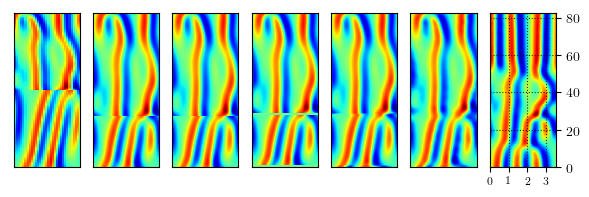
\includegraphics[width=\textwidth,height=.25\textheight]{MNG_rpo1rpo2_time}
 \end{minipage}
\caption{ \label{fig:MNGtimeglue}
Schematic demonstration of the ``gluing''  of two \twot\ solutions with
spatial translation symmetry with figures. From left to right, the
figures represent, (1) the original spatiotemporal fields combined vertically, (2) fields
with correct aspect ratio, (3) rotated fields that minimize boundary differences, (4) fields with zero padding, (5) fields with convex
buffers, (6) field with truncated spatiotemporal modes, (7) numerically
converged solution.
}
\end{figure}

\begin{figure} %[ht]
\centering
\begin{minipage}[height=.6\textheight]{.6\textwidth}
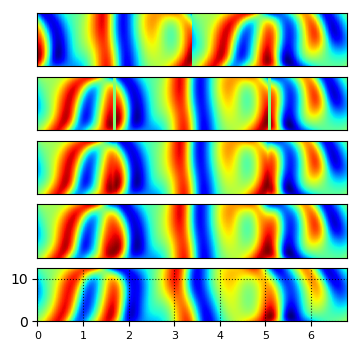
\includegraphics[width=\textwidth,height=.4\textheight]{MNG_ppo1ppo2_space}
\end{minipage}
\caption{ \label{fig:MNGspaceglue}
Schematic demonstration of spatially ``gluing''  two \twot\ solutions with shift-reflection symmetry.  From top to bottom,
the figures represent, (1) the original spatiotemporal fields side-by-side, (2) fields with zero padding, (3) fields with zero padding filled in with convex combinations
of boundaries, (4) field with truncated spatiotemporal modes, (5) numerically converged solution.
}
\end{figure}

The specific steps of the gluing process depend on the symmetry of the
initial \twots{}; currently, \twots\ that are being glued together always have the same symmetry,
and the gluing is performed in a symmetry preserving manner. The process can be summarized by
the following numbered list.

\begin{enumerate}
\item Choose two \spt\ \twot\ solutions to combine
\item Choose whether to glue spatially or temporally
\item Increase the resolution of the initial conditions by interpolation
\item Modify the discretizations to enforce the correct aspect ratio
\item (If symmetry is continuous) Rotate the two initial \spt\ fields
to minimize the difference at the gluing boundaries, ensure fields have spatial
shifts with the same sign by applying spatial reflection
\item (If symmetry is discrete) Test various combinations of fundamental domains
and choose the best combination as determined by cost function residual
\item Create zero-padding regions between the boundaries
\item Fill in the zero-padding with convex combinations of the scalar field boundaries
\item Rediscretize the final \spt\ field to reduce the number of computational
variables
\end{enumerate}

The importance of this method is that it constitutes an
alternative method for finding solutions on larger spatial
domains for this equation as well as others; three dimensional fluid
dynamics problems, for example.

\subsection{Summary of current results}
The currents results of this work include methods that find \twots\, tile \twots\, and
glue \twots\ demonstrate the computational usefulness of \spt\ methods.
The \spt\ theory, however, is currently composed of claims
and assertions that appeal to intuition. Hopefully, old theoretical machinery and
new discoveries will advance the theory to a place where rigorous and quantitative
claims can be made and proved; especially in the infinite space-time limit.
One of the main accomplishments
is the ability to find \twots\ defined on relatively large spatial domains with no
a priori knowledge other than the equations and the symmetry of the solution.
